\documentclass{nle}

\usepackage{booktabs} % For formal tables
\usepackage[utf8]{inputenc}
\usepackage{graphicx}
\usepackage{mathtools}
\usepackage{amsfonts}
\usepackage{multirow}
\usepackage{glossaries}
\usepackage{tikz}
\usepackage{pgfplots}

\DeclareMathOperator*{\argmax}{arg\,max\,}
\renewcommand{\arraystretch}{1.2}

\makeglossaries
\newacronym{nlp}{NLP}{Natural Language Processing}
\newacronym{wde}{WDE}{Web Data Extraction}
\newacronym{ner}{NER}{Named Entity Recognition}
\newacronym{hmm}{HMM}{Hidden Markov Models}
\newacronym{crf}{CRF}{Conditional Random Fields}
\newacronym{lstm}{LSTM}{Long Short-Term Memory Networks}
\newacronym{ie}{IE}{Information Extraction}
\newacronym{rne}{RNE}{Researcher Name Extraction}
\newacronym{rnn}{RNN}{Recurrent Neural Networks}
\newacronym{cnn}{CNN}{Convolutional Neural Networks}
\newacronym{pos}{POS}{Part-of-Speech}

\begin{document}

\title{Named Entity Recognition for Web Data Extraction}

% \author[João Mateus de Freitas Veneroso and Berthier Ribeiro-Neto]
%        {João Mateus de Freitas Veneroso$^A$ \and
%         Berthier Ribeiro-Neto$^B$\\
% 	Universidade Federal de Minas Gerais$^{A,B}$ \\
% 	Google Engineering$^A$, Belo Horizonte - MG, Brazil}

% \affiliation{%
%   \institution{Universidade Federal de Minas Gerais}
%   \streetaddress{Av. Pres. Antônio Carlos, 6627 - Pampulha}
%   \city{Belo Horizonte}
%   \state{MG}
%   \postcode{31270-901}
%   \country{Brazil}}
% \email{jmfveneroso@gmail.com}
% 
% \author{Berthier Ribeiro-Neto}
% \affiliation{%
%   \institution{Universidade Federal de Minas Gerais}
%   \streetaddress{Av. Pres. Antônio Carlos, 6627 - Pampulha}
%   \city{Belo Horizonte}
%   \state{MG}
%   \postcode{31270-901}
%   \country{Brazil}}
% \email{berthier@dcc.ufmg.br}
% \email{berthier@google.com}

\maketitle

\begin{abstract}

% \gls{wde} methods often rely on hand-coded rules to 
% identify and extract data from webpages. These methods are usually
% suited for extracting information from pages within
% the same website, however they perform poorly on extraction 
% tasks across different websites. Alternatively, statistical and 
% machine-learning-based sequence labeling methods provide a more flexible 
% approach to Web data extraction. Many times, HTML pages are very different 
% from plain text, because sentences are too short to provide adequate 
% context for conventional Named Entity Recognition methods to work 
% properly. Also, the HTML structure may encode information that is not 
% replicated in the text. Nonetheless, these limitations can be overcome by
% adequate feature engineering, the use of pretrained word 
% embeddings and neural character representations. In this article, we 
% evaluate the performance of different methods of named entity recognition 
% on the task of Web data extraction. In particular, we introduce a novel 
% dataset\footnote{The dataset and all models discussed in this article are 
% available in: https://github.com/jmfveneroso/ner-on-html.} 
% consisting of faculty listings from university webpages across
% the world in multiple languages and test the NER models on the task of 
% extracting researcher names from these listings. We found that a 
% neural network architecture that combines a bidirectional LSTM with
% a Conditional Random Fields output layer and LSTM-based character 
% representations outperforms other methods on the researcher name 
% extraction task, achieving an F1-score of 0.8867 with no feature engineering. 
% With the addition of hand crafted features, the F1-score can be slightly 
% improved to 0.8995.

Web Data Extraction methods often rely on hand-coded rules to 
identify and extract data from webpages. These methods are
suited for extracting information from pages within
the same website, however they perform poorly on extraction 
tasks across different websites. Alternatively, 
machine-learning-based Named Entity Recognition methods provide a more flexible 
approach to Web Data Extraction. However, many times webpages are very different 
from plain text, because sentences are too short to provide adequate 
context for conventional Named Entity Recognition models to work 
properly. 
% Nonetheless, the HTML structure also encodes useful information that 
% can be used by NER models to achieve a better performance. We propose a
% method to use this information: the self-training strategy for Hidden Markov
% Models.
In this article, we 
evaluate the performance of different methods of Named Entity Recognition
in the task of Web Data Extraction. In particular, we introduce a novel 
dataset consisting of faculty listings from university webpages across
the world in multiple languages and test different Named Entity Recognition 
models in the task of 
extracting researcher names from these listings. We found that a 
neural network architecture that combines a bidirectional LSTM with
a Conditional Random Fields output layer and LSTM-based character 
representations outperforms other methods achieving 90.2 F1 in 
the task. However, with the self-training strategy, we can get a much simpler 
model, the second-order Hidden Markov Model, to achieve 87.9 F1.

\end{abstract}

\section{Introduction}

\gls{wde} is the task of automatically extracting structured 
information from unstructured or semi-structured web documents. The input 
usually consists of web documents containing a number of predetermined entities 
organized in a similar manner. The \gls{wde} task consists of 
identifying these entities and organizing them according to a template. 

HTML documents most often lie in between the structured/unstructured 
data paradigm. DOM hierarchy, element disposition, CSS classes, and other 
features related to the document structure and indirectly associated with the 
data itself can be valuable information on the task of identifying
entities. Yet, we cannot expect these features to be completely constrained 
by an underlying pattern. Organization patterns tend to follow some guidelines 
but they are in no way subject to strict rules. That is why classical \gls{wde} 
systems such as automatic wrapper generators 
\cite{Kushmerick2000,Hsu1998,Muslea1999}
do not translate very well across different websites. 

Most existing \gls{wde} methods are tailored to extract data 
from a single webpage, producing different compromises between efficacy and 
degree of human supervision. Some unsupervised approaches proposed to tackle 
the problem of data extraction for whole application domains 
\cite{Crescenzi2001}. Usually, 
unsupervised \gls{wde} methods work in two stages. In the record segmentation stage,
WDE systems seek to cluster visually and structurally similar webpage regions 
and identify repeating data records with heuristics and 
hand-coded rules. In the attribute labeling stage, WDE systems seek to identify 
the correct attributes on data records, many times resorting to regular expressions 
or gazetteer matching strategies. The outcome of each of these stages can aid one 
another. The inner patterns of data records can help in identifying attributes of other 
data records. Also, by properly identifying data record attributes, it becomes 
easier to determine boundaries and perform record segmentation.

While unsupervised approaches can be sometimes adequate to extract information from 
webpages with similar templates, they usually fail on cross-website data extraction 
tasks. Also, more sophisticated approaches may be needed when we are not dealing
with easily distinguishable attributes such as prices and dates. 
Comparatively, statistical machine learning provides more robust and flexible methods
of \gls{wde}. In recent years, we saw amazing progress in 
the field of \gls{nlp} that is extremely relevant to
the \gls{wde} community, particularly with the introduction of Deep Neural Networks 
for Sequence Labeling~\cite{Collobert2011}, but these advancements were 
not widely incorporated by \gls{wde} systems. Also, most of the attention of the \gls{nlp} community 
regarding this topic is devoted to solving \gls{ie} tasks in plain text, such as 
the identification of people and organizations in news texts.
However, the difference between some types of webpages and plain text is significant, so
\gls{ie} systems trained in plain text datasets tend to perform poorly 
when confronted with some web extraction tasks, as we have confirmed in our experiments.

A concrete example of a \gls{wde} problem that demands the type of
flexible solution provided by statistical machine learning methods is the extraction of 
researcher names from faculty directories. Automatically extracting researcher information 
from university websites is important, for example, to construct researcher affiliation databases 
and compare the academic impact of research groups using bibliographic indices~\cite{Ribas2015}. 
The problem of \gls{rne} can be solved with machine learning methods of 
\gls{ner}.

Many \gls{wde} tasks in the web share a common
factor with the \gls{rne} task. That is, they need to extract similar
entities from different webpages or they need to extract entities from short snippets of text 
instead of complete sentences. Some examples would be comment extraction from blog
posts and \gls{ner} in tweets. Because of the lack of context in tweets, \gls{ner} methods trained 
in conventional plain text corpora tend to perform badly for more or less the same reasons 
they perform badly in other \gls{wde} tasks.

In this article, we compare different machine learning approaches to 
\gls{ner} on the web by evaluating their performance in the 
\gls{rne} task. With this purpose in mind, we introduce a novel \gls{ner} dataset 
with labeled entities, consisting of faculty directories from universities across the world. 
We compare the models in terms of their Precision, Recall, F-scores and their 
overall complexity. That is, even if a model has a slightly worse performance in terms of the
objective evaluation metrics in comparison to other approaches, it may still be useful if it 
is considerably simpler and faster to train.
The tested models were the \gls{hmm} up to third order, \gls{crf}, and a range of Deep Learning 
architectures based on Bidirectional \gls{lstm}. We also 
introduce the self-training strategy that can boost the performance 
of \gls{hmm}s in sequence labeling tasks for the web. 

The usability of the evaluated models is not limited to the particular problem of \gls{rne}. 
By reliably detecting named entities on the web, we can boost the performance 
of existing \gls{wde} approaches or even construct an end-to-end architecture that
solves the problem of data extraction across different websites with improved robustness. Also, 
the researcher affiliation database constructed with the application of these methods will
be made public in the future to provide deeper insight in bibliometric studies about the
scientific impact of research groups.


\section{Related Work}
\label{cha:related_work}

The \gls{rne} task is a problem in \gls{wde} that
we proposed to solve with the application of machine learning methods of \gls{ner}.
This chapter presents the related research in the fields of \gls{wde} 
in Section~\ref{sec:wde} and \gls{ner} in Section~\ref{sec:ner}.

\subsection{Web Data Extraction}
\label{sec:wde}

Since the early 1990s, the astonishing growth of public information in the web has 
led to the development of a number of different approaches to the problem of \gls{wde}.
Traditionally, the task was solved by designing special purpose
programs called wrappers to recognize relevant data and store records in a structured
format. These early tools varied wildly relative to their degree of automation. 

It was readily perceived that manual wrapper generation was a rather tedious and
error prone process, unsuited for large scale operations. Wrappers tend to
break frequently because they rely on webpage features that can change 
often. So, in the late nineties, several authors advocated for wrapper induction, a technique 
that consists of automatically constructing wrappers from a small set of examples by 
identifying delimiters or context tokens that single out the desired attributes. 
Some remarkable wrapper induction methods are WIEN~\cite{Kushmerick2000}, Soft 
Mealy~\cite{Hsu1998} and STALKER~\cite{Muslea1999}.

Despite being better than constructing wrappers manually, wrapper induction methods 
still suffered from a lack of expressive power and flexibility. These methods had 
trouble handling records with missing attributes or unusual structures because
patterns could only be identified if they happened at least once in the examples.

Other approaches such as NoDoSE~\cite{Adelberg1998} and Debye~\cite{Laender2002a} 
brought greater flexibility to wrapper induction methods by requiring a greater level 
of human interaction through graphical user interfaces. \gls{wde} techniques often 
require some sort of assistance from human experts to boost accuracy. One of the main challenges 
in the field lies in determining an adequate trade-off between the degree of automation and 
the Precision and Recall of the data extraction tool.

To automate the task of \gls{wde} completely some approaches,
such as Road Runner~\cite{Crescenzi2001}, removed entirely the need for data examples.
Road Runner parses documents belonging to a same class (e.g. books in Amazon) and 
generates wrappers based on their similarities and differences, yielding comparable results 
to those obtained by wrapper induction methods. However, like previous approaches, it was 
unsuited for cross site extraction tasks because the learned rules were not general enough.

Early NLP-based approaches aimed at extracting more general rules that could possibly
be employed over multiple websites. RAPIER~\cite{Califf1999} is a method of rule
extraction that uses information such as part-of-speech tags and semantic classes from
a lexicon to derive patterns from a set of training examples. This approach is more
flexible than the wrapper induction methods, however it achieves much lower rates of 
Precision and Recall.

A survey by Laender, Ribeiro-Neto, da Silva and Teixeira~\shortcite{Laender2002b} made a thorough classification of the
early approaches with a taxonomy based on their main technology, being them: languages for
wrapper development, HTML-aware tools, NLP-based tools, Wrapper Induction Tools,
Modeling-based tools and Ontology-based tools. Some noteworthy examples from this era
are: 
%
\begin{itemize}
\item TSIMMIS~\cite{Hammer1997} and WebOQL~\cite{Arocena1999}, which are special purpose 
languages for building wrappers.
\item Road Runner~\cite{Crescenzi2001}, XWRAP~\cite{Liu2000} and W4F~\cite{Sahuguet1999}, 
which are HTML-aware tools that infer meaningful patterns from the HTML structure.
\item RAPIER~\cite{Califf1999}, SRV~\cite{Freitag1998}, WHISK~\cite{Soderland1999}, which 
are NLP-based tools.
\item WIEN~\cite{Kushmerick2000}, Soft Mealy~\cite{Hsu1998} and STALKER~\cite{Muslea1999} which 
are wrapper induction methods.
\item NoDoSE~\cite{Adelberg1998} and Debye~\cite{Laender2002a}, which are semi-supervised
tools that require some interaction with the user by means of a graphical
user interface.
\end{itemize}
%
% Text Runner.
% https://www.aaai.org/Papers/IJCAI/2007/IJCAI07-429.pdf
\cite{Chang2006} complemented the previous surveys with semi-supervised 
technologies such as Thresher~\cite{Hogue2005}, IEPAD~\cite{Chang2001} and 
OLERA~\cite{Chang2004}. They differed from supervised 
and unsupervised methods because they either needed only a rough description of
data from users for extraction rule generation or some level of post processing
that needed user attention. 
%The survey also mentioned newer unsupervised methods
% such as DeLa~\cite{Wang2003}, Exalg~\cite{Arasu2003} and Depta~\cite{Zhai2005}.

Most of the early \gls{wde} systems were rule-based with either 
manual rule description or automatic rule learning from examples, thus they
suffered from a lack of flexibility when dealing with noisy and unstructured data.
Huge progress in the field of statistical learning led to the development of
models that tried to solve this problem.

\cite{Sarawagi2008} introduced a classification that segmented wrappers in
rule-based methods, statistical methods and hybrid models, bringing together 
the fields of \gls{ner}, Relationship Extraction and \gls{wde}. 
The rule based methods encompass most of the previous models. While the statistical methods 
convert the extraction task into a token labeling task, solved with \gls{ner} 
and Relationship Extractions methods. Traditionally, these subtasks were solved with 
generative models based on \gls{hmm}s or discriminative models based on the 
Maximum Entropy principle, but recently these have been largely superseded by Deep Neural 
Networks. Different from automatic wrapper generators, statistical methods are suitable for
a large variety of tasks, especially when we want the system to handle cross website information 
extraction and plain text information extraction. That is why this class of methods is of 
special interest to our application. The progress of statistical models will be 
discussed in Section~\ref{sec:ner}.

Surveys by~\cite{Ferrara2014}, \cite{Schulz2016} and \cite{Varlamov2016} updated the 
previous surveys on Information Extraction methods with some interesting innovations. 
Some examples are: the Visual Box Model~\cite{Krupl2005}, a data extraction system that produces 
a visualization of the webpage to exploit visual cues to identify records presented in a tabular form;
automatic wrapper adaptation~\cite{Ferrara2011}, a technique that tries to reduce the cost of 
wrapper maintenance by measuring the similarity of HTML trees and adapting
wrappers to the new page structure; AutoRM~\cite{Shi2015}, a method to mine
records from a single webpage by identifying similar data regions through DOM
tree analysis; and Knowledge Vault~\cite{Dong2014}, a method that combines different 
extraction approaches to feed a probabilistic knowledge base.

Most data extraction systems focus on extracting information from single websites
and are therefore unsuited for cross website extraction tasks. Even unsupervised
approaches that are application domain independent, such as RoadRunner and EXALG, 
only work well when extracting data from pages generated from a same template. 

A statistical approach to unsupervised domain 
independent \gls{wde} was described by~\cite{Zhu2005}. The 2D CRF 
model takes a webpage segmented into data blocks and employs a two dimensional \gls{crf}
model to perform attribute labeling. The model was further improved 
in~\cite{Zhu2006} to model record segmentation and attribute labeling as a joint task.
Some of the limitations of early unsupervised methods 
were also addressed by ObjectRunner~\cite{Abdessalem2010} and DIADEM~\cite{Furche2012}. 
These methods work by annotating webpages automatically with regular expressions, gazetteers and 
knowledge bases. They can rectify low quality annotations and even improve the annotators
by exploring regular structures in the DOM during the record segmentation phase.

\gls{wde} methods have undoubtedly improved extraordinarily, but
as pointed by \cite{Schulz2016}, it is difficult to compare the results 
achieved by competing tools. Also, many tools seem to rely excessively on heuristic methods.
The recent advancements in sequence taggers may provide more robust and flexible techniques
to address this problem.


\subsection{Named Entity Recognition}
\label{sec:ner}

\gls{ner} is an important subtask in \gls{ie}.
The \gls{ner} task was defined in the Third Message 
Understanding Conference (MUC-3)~\cite{Sundheim1991}, where researchers were asked to extract
entities from a news corpus about terrorist incidents. However, it was the 
language-independent \gls{ner} shared task at the Conference 
on Computational Natural Language Learning in 2003 ({CoNLL-2003})~\cite{KimSang2003},
that established an enduring labeled dataset constructed with news texts from Reuters.
Despite its reduced size and the limited variability of its documents, the {CoNLL-2003}
dataset is still used to compare the performance of NER systems in English and 
German. 

Sequence labeling for \gls{ner} and \gls{pos} tagging (labeling nouns, verbs, pronouns, etc.) 
is very similar, so, many times, research articles that propose new methods for \gls{ner}
also report results for the \gls{pos} Tagging task. And frequently, the best methods for 
\gls{pos} Tagging are also the best methods for \gls{ner}.

Traditionally, the \gls{ner} task was solved with generative models based on 
\gls{hmm}s. The first appearance of \gls{hmm}s in the
field of \gls{nlp} occurred in the mid-seventies and was
primarily focused on the problem of Speech Recognition. 
But in the late nineties, \gls{hmm}s also found important applications in \gls{ie}
and \gls{ner} as in the works by~\cite{Bikel1999}, 
\cite{Freitag1999}, and \cite{Freitag2000}.

The problem with \gls{hmm}s is that they model the joint probability between 
sequences of observations and labels $ P(X, Y) $, a harder problem than modelling the corresponding 
conditional probability $ P(Y|X) $. They assume conditional independence for the observations $ X $, and
therefore, they cannot handle overlapping features. This lack of flexibility led to the 
development of discriminative approaches to sequence labeling based on the Maximum Entropy principle.

Some early examples are Maximum Entropy Taggers for NER~\cite{Borthwick1998} and
\gls{pos} Tagging~\cite{Ratnaparkhi1998}. The Maximum Entropy Markov Model~\cite{McCallum2000} 
was developed just a while later, building up on the intuition of \gls{hmm}s combined with
the flexibility of discriminative approaches. However, because of the label bias problem,
this model was superseded by \gls{crf}s~\cite{Lafferty2001, McCallum2003}. 
At this time, the best performing systems almost always resorted to external gazetteers 
and hand-chosen features, as is the case for the {CoNLL-2003} winning model~\cite{Florian2003}.

With the advancement of Machine Learning in recent years, we saw the rise
of Neural Networks applied to sequence labeling. In 2011, \cite{Collobert2011} 
introduced Neural Networks free of feature engineering to sequence labeling tasks,
using \gls{cnn} over word embeddings with a CRF output layer to tackle 
the problems of \gls{pos} tagging, Chunking, Semantic Role Labeling, and NER. A similar architecture 
proposed in 2015 by~\cite{Huang2015}, the Bi-LSTM-CRF, replaced the \gls{cnn} in \cite{Collobert2011} 
with a bidirectional LSTM, achieving better results.

In 2016, further advancement to the NER models was achieved by incorporating character 
representations at the bottom of the Bi-LSTM-CRF architecture to extract morphological 
features from words automatically. The model by~\cite{Lample2016} uses a 
bidirectional \gls{lstm} over character embeddings and the model by~\cite{Ma2016} uses a
one dimensional \gls{cnn} with max pooling over character embeddings. Both models also 
made use of pre-trained GloVe word embeddings, created by~\cite{Pennington2014}.

Small improvements to NER systems have been made since then, primarily due to the 
introduction of new word embeddings on variations of the Bi-LSTM-CRF architecture. From
this group, we can mention ELMo~\cite{Peters2018}, BERT~\cite{Devlin2018}, and
Flair~\cite{Akbik2018}. 
All of them were introduced in 2018 and they differ primarily 
in how to construct contextual embeddings from the internal states of a language 
modelling neural network.

To our knowledge, the best NER system up to this date (considering the performance in the
{CoNLL-2003} dataset) is the bidirectional transformer model proposed by~\cite{Baevski2019} that uses
a stack of self-attention modules and ELMo embeddings. Table~\ref{tab:ner_model_comparison}
shows a comparison of the history of reported F1 scores in the English test set of the {CoNLL-2003} dataset
for the NER systems that were mentioned in this section. Each of the mentioned systems held the 
record for the task at a given time.

\begin{table}[h]
  \small
  \begin{center}
    \begin{tabular}{ lc }
      \toprule
      Model & Test F1 \\
      \midrule
       \cite{Florian2003} ({CoNLL-2003} Winner)    & 88.76 \\
       \cite{Collobert2011}                        & 89.59 \\
       \cite{Huang2015}                            & 90.10 \\
       \cite{Lample2016}                           & 90.94 \\
       \cite{Ma2016}                               & 91.21 \\
       \cite{Peters2018}                           & 92.22 \\
       \cite{Devlin2018}                           & 92.80 \\
       \cite{Akbik2018}                            & 93.09 \\
       \cite{Baevski2019}                          & 93.50 \\
      \bottomrule
    \end{tabular}
  \end{center}
  \caption{Model performances in the {CoNLL-2003} English test set.}
  \label{tab:ner_model_comparison}
\end{table}

\section{Named Entity Recognition Models}

Many \gls{wde} systems rely on hand crafted rules or gazetteers to perform
attribute annotation. Machine learning approaches to NER can improve annotations of 
more complex entities and even perform entity detection without any feature
engineering. We explored many methods of Named Entity Recognition
in the context of a \gls{wde} task. First, we discuss two traditional 
approaches: Hidden Markov Models, and Linear Chain Conditional Random Fields. Then,
we discuss neural network architectures.

\subsection{Hidden Markov Models}

A Markov Model is a stochastic model that computes the most probable sequence of states 
given a limited set of observable states $ S = \{s_1, s_2, ..., s_n \} $.
The Hidden Markov Model (HMM) differs from the Markov Model in that it
does not observe the states directly, but rather a probabilistic function of those 
states. For example in NER, the words are observed, however the Named Entity labels
associated with these words are not. Formally, we want to compute the most probable
sequence of labels $ Y = \{y_1, y_2, ..., y_n\} $ for a sequence of observed tokens
$ X = \{x_1, x_2, ..., x_n\} $.

\begin{equation}
Y^* = \argmax_{Y} P(Y|X)
\end{equation}

With Bayes theorem, we can write $ P(Y|X) $ as:

\begin{equation}
P(Y|X) = \frac{P(X|Y) P(Y)}{P(X)}
\end{equation}

Since $ P(X) $ is the same for all label sequences $ Y $, we can simply maximize
the probability $ P(X|Y) P(Y) $.

A HMM makes two assumptions. First, the probability of being in a given state depends 
only on a fixed number of previous states. That is:

\begin{equation}
P(y_i|y_{i-1}x_{i-1}, y_{i-2}x_{i-2}, ..., y_1x_1) = P(y_i|y_{i-1}, y_{i-2},..., y_{i-k})
\end{equation}

In fact, we can get much better results on the NER task by looking at trigrams
or quadrigrams ($ k = 2 $ or $ k = 3 $) instead of bigrams as with a regular HMM. 
Some label assignments are highly improbable, such as single token named entities 
separated by a common word. These kinds of patterns can be perceived by a higher order HMM.
Second, the probability of a word depends only on its assigned label. That is:

\begin{equation}
P(x_i|y_{i-1}x_{i-1}, ..., y_1x_1) = P(x_i|y_i)
\end{equation}

With these assumptions, 
the probability $ P(Y|X) $ can be approximated by the expression:

\begin{equation}
P(Y|X) \propto \prod_{i=k+1}^{n} P(y_i|y_{i-1}, y_{i-2}, ..., y_{i-k}) P(x_i|y_i)
\end{equation}

All relevant probabilities can be estimated through maximum likelihood estimation from the relative
frequencies of labels and features in the corpus. The best sequence of labels can be computed 
with a variable state Viterbi approach \cite{Li2000}. However, as we increase $ k $, this computation 
becomes exponentially more expensive. The beam-search strategy may be employed for a faster 
search, but we found that for $ k \leq 4 $, the Viterbi algorithm is still viable.

HMM based taggers have been successfully applied in many NLP and WDE tasks 
\cite{Rabiner1990,Freitag2000}. They are incredibly fast to train and also they are very 
interpretable, making them a good choice for a first approximation. However, these models 
are highly dependent on the right selection of features, what may outweigh the benefit of a 
small training cost.

\subsubsection{Self-Training for Hidden Markov Models} 
\label{sssec:self_training}

As described in Section~\ref{sec:hmm}. An \gls{hmm} for the sequence labeling task 
has the form:
\begin{equation}
P(Y|X) \propto \prod_{i=1}^n P(x_i|y_i) P(y_i, y_{i-1})
\end{equation}
where $ X $ is a sequence of words and $ Y $ is a sequence of labels, both with size $ n $,
and the initial probabilities $ P(y_1|y_0) $ follow a uniform distribution across all label 
assignments.
To construct this model from the data, we need to estimate the following probabilities:
%
\begin{itemize}
  \item $ P(x_i|y_i) $: the emission probability of word $ x_i $ given label $ y_i $.
  \item $ P(y_i|y_{i-1}) $: the transition probability of going from label $ y_{i-1} $ to label $ y_i $.
\end{itemize}
%
We may consider $ x_i $ to be a binary feature vector $ x_i = \{ f_{i,1}, f_{i,2}, ..., f_{i,k} \} $
as long as all the feature distributions are independent, conditioned on $ y_i $. That is:
\begin{equation}
P(x_i|y_i) = P(f_{i,1}, f_{i,2}, ..., f_{i,k}|y_i) = \prod_{j=1}^k P(f_{i,j}|y_i)
\end{equation}
%
Also, due to the time invariance assumption, the $ P(f_{i,j}|y_i) $ probabilities 
are independent of the timestep $ i $. Therefore, for each binary feature $ f_j $ we
need only estimate the parameters $ \hat{P}(f_{j}|y) $, relative to each possible
assignment of $ y $.
The maximum likelihood estimators for these feature parameters can be obtained
from their relative frequencies, just as we did in Section~\ref{sec:hmm} for single words 
(Equation~\ref{eq:mle_words}). Then, for binary features:
%
\begin{equation}
\hat{P}(f_{j}=1|y=l) = \frac{\text{Count}(f_{j}=1, y=l)}
{\text{Count}(f_{j}=0, y=l) + \text{Count}(f_{j}=1, y=l)}
\label{eq:feature_mle}
\end{equation}
%
Where $ \text{Count}(f_{j}=1, y=l) $ is the number of times in the training set that
feature $ f_j $ was equal to one when the actual label was $ l $ (the other counts follow the same logic).
This approach yields good experimental results for textual features such as the capitalization
of a word, but if we try to use HTML structural features such as the HTML tags, we will find that
they are not very useful, contradicting our intuition.
The problem is that there is not much similarity between the HTML structure in different web pages.
For example, only because a named entity label occurs more often inside <div> tags
in a page, that does not mean this is the case for most web pages. Consider for example a faculty web page 
that shows researcher names in a table (<td> tags) in contrast to a web page that organizes researcher
names in a list (<li> tags). If there are many cases like the former page in our training set, and we use the 
HTML tag feature in a model that assigns labels to the latter page in our test set, we will probably get many 
wrong predictions.
Nonetheless, the HTML features are not useless. Inside a single web page, the HTML tag is a good predictor
of the correct labels. Words with a similar HTML context tend to have similar labels. For example, words
that happen together in a list have very similar HTML contexts and are very likely to belong to
the same category. The question is how to obtain better parameter estimators for HTML features.

Consider a set $ F^T $ of $ m $ textual features unrelated to the HTML structure:
%
\begin{equation*}
F^T = \{ f^T_1, f^T_2, ..., f^T_m \}
\end{equation*}
%
And a set $ F^H $ of $ k $ HTML features that are related to the HTML structure:
%
\begin{equation*}
F^H = \{ f^H_1, f^H_2, ..., f^H_k \}
\end{equation*}
%
Given a \gls{hmm} trained with only the first set of features $ F^T $,
we can use this model to predict the labels for an unlabeled document, and then by simply replacing
the actual labels in Equation~\ref{eq:feature_mle} with the predicted labels, we get:
%
\begin{equation}
\hat{P}(f_{j}=1|y=l) = \frac{\text{Count}(f_{j}=1, \tilde{y}=l)}
{\text{Count}(f_{j}=0, \tilde{y}=l) + \text{Count}(f_{j}=1, \tilde{y}=l)}
\end{equation}
%
\begin{equation}
\hat{P}(\text{Tag}=\text{<li>}|y=\text{I-PER}) = \frac{4}{4 + 0} = 1
\end{equation}
%
Where $ \tilde{y} $ is the label predicted by the \gls{hmm} trained with only the textual features.
We use this formulation to calculate feature probabilities for the HTML features only.
And next, we incorporate the estimators for the HTML feature probabilities in the original \gls{hmm} 
and predict the final labels with the whole set of features $ F^T \cup F^H $. 
This process could be repeated multiple times. If the predictions are becoming more accurate with
each iteration, then the estimates for the HTML feature probabilities are also likely to improve. 

In a simpler explanation, the self-training strategy can be divided into the following steps:
%
\begin{itemize}
\item Train the HMM without any HTML features.
\item Compute labels for a website with the trained HMM.
\item Use the computed labels as a proxy for the actual labels in the 
website and estimate HTML feature frequencies for this website alone.
\item Recompute the labels now using the HTML feature probabilities.
\end{itemize}
%
To understand why this strategy could help labeling named entities on the web, consider the 
example shown in Figure~\ref{fig:self_training}. This example shows a snippet from a webpage 
and how a naive \gls{hmm} would probably attribute 
labels to each word. Despite being rather uncommon, North West is an actual person name,
what becomes obvious in this case once we know the HTML context where it happens 
(inside a list with other person names), but this is not so obvious if we consider the
sentence in isolation. The naive \gls{hmm} could be improved if we calculated
feature probabilities for the parent tags using proxies for the correct labels. We would find
that four times in a total of six occurrences, the correct label for a word that happened inside
a \textit{<li>} tag was \mbox{\textit{I-PER}}. By incorporating this knowledge in the model 
using the self-training strategy, we would improve the probability that words North and West 
were labeled correctly as a person name in this case.

\begin{figure}
  \centering
  \includegraphics[width=0.5\textwidth]{pics/self_training_example}
  \caption{Example of a webpage snippet with labels attributed by a HMM.}
  \label{fig:self_training}
\end{figure}

This strategy could possibly be incorporated in the Baum-Welch algorithm to provide a more 
statistically solid argument for its effectiveness, but this heuristic
already yields a consistent improvement to sequence labeling on the web. In theory, this 
strategy could be used with any sequence tagger, however retraining a classifier with new features can 
become prohibitively expensive in the case of CRFs or Neural Networks. 
In HMMs, retraining the features
is fast, because we assume feature independence and the maximum likelihood estimator can be 
obtained with a simple closed form expression.


% \subsubsection{Self training} 
% \label{sssec:self_training}
% 
% In the task of NER on HTML, there are useful features related to the HTML
% structure that can help in identifying named entities. In a given website, named
% entities tend to occur inside the same HTML tags. The HTML tag feature or other
% HTML features could easily be incorporated in the HMM. However, these 
% features are only useful inside a single website and they cannot be generalized, 
% because different websites use distinct HTML templates. 
% Therefore, we propose a self-training strategy to obtain probabilities for
% these HTML features. It is implemented like this:
% 
% \begin{itemize}
% \item Train the HMM without any HTML features.
% \item Compute labels for a website with the trained HMM.
% \item Use the computed labels as a proxy for the actual labels in the 
% website and estimate HTML feature frequencies for this website alone.
% \item Recompute the labels now using the HTML feature probabilities.
% \end{itemize}
% 
% In theory, this strategy could be used with any sequence tagger, however
% retraining a classifier with new features can become prohibitively expensive.
% This strategy is only possible because the computation of HTML feature
% frequencies can be performed very quickly. This adds very little overhead 
% to the original HMM and improves precision and recall by a considerable 
% margin.

\subsection{Linear Chain Conditional Random Fields}

A Linear Chain Conditional Random Field (CRF) is the discriminative analog to the HMM,
it was first introduced by Lafferty \cite{Lafferty2001}. It is a distribution $ P(Y|X) $ that takes the form:

\begin{equation}
P(Y|X) = \frac{1}{Z(x)} \prod_{t=1}^{T} exp \left( \sum_{k=1}^{K} \theta_k f_k(y_{t-1}, y_t, X) \right)
\end{equation}
\\

where $ \theta $ is the parameter vector that we are going to learn, $ f_k(y_{t-1}, y_{t}, X) $ 
are feature functions over the current timestep $ t_y $, the previous timestep $ y_{t-1}$, 
and the observation vector $ X $. And the partition function $ Z(x) $, takes the form:

\begin{equation}
Z(x) = \sum_{Y} \prod_{t=1}^{T} exp \left( \sum_{k=1}^{K} \theta_k f_k(y_{t-1}, y_t, x) \right)
\end{equation}
\\

which is a sum over all possible label assignments $ Y $. The partition function can be efficiently
and exactly calculated with the sum-product algorithm. Parameter estimation is usually done through 
negative log likelihood minimization. The function can be optimized with techniques suitable for other 
maximum entropy models such as L-BFGS \cite{Liu1989}. The most likely label sequences can be decoded 
with the Viterbi algorithm, as was the case for HMMs.

CRFs are more general than HMMs because the transitions from $ y_{t-1} $ to $ y_{t} $ can depend 
on the whole vector of observations $ X $. This flexibility of feature functions allows for a wide range of
possibilities. Recently, CRFs have been successfully employed as the output layer in complex neural 
architectures bringing improvements over models that compute labels independently.

\subsection{Neural Network Architectures}

Recurrent neural networks (RNN) have been successfully employed on numerous NLP tasks such as
language modelling, POS tagging, speech recognition and NER. Different from feed-forward 
neural networks, RNNs can retain information in their internal state, making them more 
suitable for processing sequences, and consequently for solving text related tasks. 
Figure~\ref{fig:rnn_network} describes an RNN for sequence labeling unrolled through multiple 
timesteps. 

\begin{figure}[h]
  \centering
  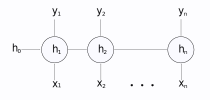
\includegraphics[width=0.75\textwidth]{pics/rnn_network}
  \caption{RNN for NER}
  \label{fig:rnn_network}
\end{figure}

At each timestep, the neural network computes a hidden state $ h_t $ using an input 
vector $ x_t $ and the previous hidden state $ h_{t-1} $, that retains information from past 
iterations. Finally, the RNN produces an output vector $ y_t $ representing the label for that 
timestep. A common definition for an RNN cell is given by the equations:

\begin{flalign*}
h_t &= tanh(W_x x_t + W_h h_{t-1}) &\\
y_t &= softmax(W_y h_t) &
\end{flalign*}

Where $ W_x $, $ W_h $ and $ W_y $ are weight matrices that can be trained with the 
Backpropagation Through Time (BPTT) algorithm. Theoretically, RNNs are capable of learning
and retaining long term dependencies through their internal state $ h_t $. However, in practice,
it becomes difficult due to the vanishing gradient problem. Long short term memory networks (LSTM) were 
introduced by Hochreiter and Schmidhuber \cite{Hochreiter1997} with this problem in mind and 
have been popularized since then. 

LSTMs incorporate a memory cell $ c $ in the RNN definition and three gates to control 
the flow of information that comes in and out of the memory cell.
The input gate $ \Gamma_{i} $ controls the amount of new information that will flow into the memory cell,
the forget gate $ \Gamma_{f} $ controls the amount of previous information that will be retained in the memory
cell, and the output gate $ \Gamma_{o} $ controls the amount of information stored in the memory cell that
will be used to compute the output activation of the LSTM unit. 
LSTM cell implementations vary slightly in the literature. A visual description of 
our LSTM cell is provided in Figure~\ref{fig:lstm_cell}.

\begin{figure}[h]
  \centering
  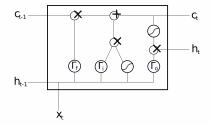
\includegraphics[width=0.75\textwidth]{pics/lstm_cell}
  \caption{LSTM Cell}
  \label{fig:lstm_cell}
\end{figure}

The equations for the LSTM cell are:

\begin{flalign*}
\Gamma_{i} &= \sigma(W_i \cdot [x_t,h_{t-1}] + b_i) &\\
\Gamma_{f} &= \sigma(W_f \cdot [x_t,h_{t-1}] + b_f) &\\ 
\Gamma_{o} &= \sigma(W_o \cdot [x_{t},h_{t-1}] + b_o) &\\
c_t        &= \Gamma_{f} \ast c_{t-1} + \Gamma_{i} \ast tanh(W_c \cdot [x_{t},h_{t-1}] + b_c) &\\
h_t        &= \Gamma_{o} \ast tanh(c_t) &
\end{flalign*}

Where $ \sigma $ is the logistic sigmoid function. $ \Gamma_i $, $ \Gamma_f $, and $ \Gamma_o $ are the input,
forget and output gates, respectively, and $ W_i $, $ W_f $, $ W_o $ are the weight 
matrices corresponding to each gate. $ c_{t} $ is the cell 
state at time $ t $ and $ h_{t} $ is the hidden state at time $ t $. 
The vector $ [x_{t},h_{t-1}] $ is formed by concatenating the current input vector 
$ x_{t} $ and the hidden vector from a previous timestep $ h_{t-1} $. Finally,
$ A \ast B $ represents the element-wise multiplication of matrices $ A $ and $ B $
and $ A \cdot B $ represents the dot product of $ A $ and $ B $.

This implementation differs from the LSTM cell described in Huang et al. \cite{Huang2015}
in that the gates $ \Gamma_i $ and $ \Gamma_f $ do not receive inputs from the previous 
cell state $ c_{t-1} $ and the output gate $ \Gamma_{o} $ does not receive inputs from the current cell 
state $ c_{t} $. This variation produces little difference in terms of model accuracy on
the performed task, but it reduces model complexity.

\subsubsection{BI-LSTM-CRF}
\label{sssec:lstm_crf}

On named entity recognition tasks, both past and future words are important 
to attribute a label at time $ t $, however a regular LSTM network only takes 
past states into consideration. A bidirectional LSTM solves this problem by stacking 
two regular LSTMs, and feeding them with observations in opposite directions. The first LSTM 
receives forward states and the second LSTM receives backward states. The hidden states from both 
networks can then be concatenated at each timestep to produce output labels. With this 
architecture, LSTM cells may use information from past and future timesteps to decide 
the label at time $ t $.

Huang et al. \cite{Huang2015} proposed a bidirectional LSTM with a CRF layer (BI-LSTM-CRF) on 
the output to tackle the sequence tagging problem. The main benefit of adding a CRF layer 
in the neural sequence model is that the labels are jointly decoded for a whole sentence 
instead of being predicted individually. Another possibility would be to use a beam search
decoder to find an optimal sequence of labels. Predicted tags should be highly correlated 
in a named entity recognition task, so it is desirable to predict sequences conjointly.
The BI-LSTM-CRF is described in Figure~\ref{fig:bi_lstm_crf}.

\begin{figure}[h]
  \centering
  \includegraphics[width=0.75\textwidth]{pics/bi_lstm_crf}
  \caption{Bidirectional LSTM-CRF}
  \label{fig:bi_lstm_crf}
\end{figure}

This architecture achieved an F1 score of 90.10 on the English data from the CoNLL-2003 
NER shared task \cite{KimSang2003}, in contrast to 85.17 for a bidirectional LSTM without 
a CRF layer. 
In our experiments, the LSTM-CRF architecture uses a bidirectional LSTM with 100 
hidden states, no peepholes and input and output dropout layers with a dropout
rate of 0.5. The dropout layers have proven to be very important to prevent overfitting 
and allow better generalization.

\subsubsection{CNN character representations}
\label{sssec:lstm_crf_cnn}

Ma and Hovy \cite{Ma2016} proposed to add a convolutional neural network (CNN) layer 
on top of a bidirectional LSTM-CRF to encode character-level information. The CNN
layer is described visually in Figure \ref{fig:cnn}.

\begin{figure}[h]
  \centering
	  \includegraphics[width=0.75\textwidth]{pics/cnn}
  \caption{CNN based character representations}
  \label{fig:cnn}
\end{figure}

The convolutional neural network receives character embeddings as inputs. The character 
representations generated by the CNN are combined with word level representations 
and fed to the BI-LSTM-CRF described in section \ref{sssec:lstm_crf}.
This architecture can learn morphological features that are very
useful in the NER task, since similar named entities often present morphological similarities. 
This architecture obtained an F1 score of 91.21 in the CoNLL2003 dataset. In our experiments, 
the LSTM-CRF architecture with CNN character representations uses a one dimensional convolutional 
neural network with 30 filters and a window size of three characters on top of the LSTM-CRF 
architecture. The character embeddings fed to the CNN have 30 dimensions that are randomly 
initialized.

\subsubsection{LSTM character representations}

Lample et al \cite{Lample2016} proposed to use a bidirectional LSTM to model character-level 
representations on top of a BI-LSTM-CRF. Combining the forward and backward LSTM hidden states 
to form the character representation, as described in Figure~\ref{fig:lstm_char}. 

\begin{figure}[h]
  \centering
  \includegraphics[width=0.75\textwidth]{pics/lstm_char_representations}
  \caption{LSTM based character representations}
  \label{fig:lstm_char}
\end{figure}

This character representation is also combined with a word 
representation and fed to a BI-LSTM-CRF network. 
The forward state is expected to be a better representation of the suffix of 
a token, and the backward state is expected to be a better representation of 
the prefix of a token. This differentiates the architecture
from the CNN based approach described in Section~\ref{sssec:lstm_crf_cnn}, because CNN filters 
discover positional invariant features, while LSTMs can better represent 
suffixes and prefixes. In our experiments, 
the LSTM-CRF architecture with LSTM character representations was implemented with a bidirectional 
LSTM with 25 hidden states, producing character representations of 
size 50. The character embeddings have 30 dimensions that are randomly initialized.

\subsubsection{Network training}

All neural models were trained using mini batch Stochastic Gradient Descent over 50 epochs with batch size 10,
learning rate 0.01, momentum 0.9 and decay rate 0.05. We used early stopping \cite{Caruana2000} to select the best 
parameters, considering the F1 measure in the validation set. All neural models used 
GloVe 100-dimensional word embeddings \cite{Pennington2014} that were fine tuned during training.
In the case of NER on HTML, word embeddings work similarly to a gazetteer. Named entities 
with the same type have similar embeddings, so good word embeddings can achieve exceptional 
performance with little training and without a gazetteer. 

\section{Researcher Name Extraction Dataset}
\label{cha:dataset}

This chapter describes the dataset used to evaluate the performance of sequence labeling models
on the \gls{wde} task of \gls{rne}. We call it the \gls{rne} dataset.
We attested experimentally that 
models trained in a popular \gls{ner} dataset (the {CoNLL-2003} English dataset) do not perform 
well in the \gls{rne} task and this is likely due to the differences
between plain text and HTML. The lack of other \gls{ner} 
datasets built for HTML name extraction imposes the need to construct a dataset specific for \gls{rne}.

The \gls{rne} task consists of finding researcher names in faculty listings from university 
webpages across the world, mainly from Computer Science departments.
This would be a necessary step when linking researcher profiles from university 
websites to their entries in public databases. Unlike many
\gls{wde} datasets, each webpage in the \gls{rne} dataset comes from a different 
website, and therefore has a different format, what makes many \gls{wde}
approaches impractical. The idea is to explore systems that are general 
enough to allow accurate entity extraction from different sources while requiring
no supervision between different websites. 

We collected 145 Computer Science and Engineering faculty pages from 42 different countries in
multiple languages, although the English version was preferred when it was available.
We gathered faculty webpages in proportion to
the number of universities in each country\footnote{A detailed list of universities can
be found in https://univ.cc/world.php}. 
The dataset size was limited to a number of pages that could be viably labeled manually and
that could still represent many different countries. 
Also, university pages that contained 
corrupt HTML or JavaScript code that performed lazy loading of data records were
not included in this dataset.

This chapter is divided as follows. Section~\ref{sec:data_description} describes the 
dataset format and how it was split in
three data files. 
Section~\ref{sec:evaluation} describes how the evaluation of results in this 
dataset was carried on. 
Section~\ref{sec:dictionary} describes how we obtained a dictionary
of relevant named entities for this dataset, and discusses some baselines.
Lastly,
Section~\ref{sec:conll_comparison} compares the characteristics of the \gls{rne} dataset
with another popular \gls{ner} dataset, the {CoNLL-2003} English \gls{ner} dataset.

\subsection{Data Description} 
\label{sec:data_description}

Each of the 145 faculty pages was preprocessed and converted
to the {CoNLL-2003} data format. That is, one word per line with empty lines representing
sentence boundaries. Sentence boundaries were determined by line break HTML tags
(div, p, table, li, br, etc.) in contrast to inline tags (span, em, a, td, etc.). For example,
the HTML sentence: 
%
\begin{quote}
\centering
<p>E. <b>Smith</b> is a <a href="/link">professor</a>.</p>
\end{quote}
%
\noindent
becomes:
%
\begin{quote}
\centering
E. Smith is a professor.
\end{quote}
%
Sentences that were more than fifty tokens long were also split according to the
punctuation. Some algorithms have trouble handling very big sentences, so we verified
experimentally that fifty tokens provide a large enough context 
and allow efficient training using a GPU. A few sentences in the dataset would be 
more than a thousand tokens long if this step was not performed, what would make batch training
for neural networks less efficient.

% The algorithm used for sentence segmentation is described in
% Appendix~\ref{app:html_segmenter}.

A robust tool for HTML segmentation poses many challenges by itself, but the simple approach 
adopted here has proved to be sufficient to perform \gls{rne} adequately. 
Also, it is best to evaluate \gls{ner} models without relying on any sophisticated data 
record segmentation system.
In many cases, entity annotation may precede the segmentation
phase on \gls{wde} methods. Also, depending on the task (as is the case
for researcher name extraction), a good annotator that is able to work 
with raw HTML provides a good solution to the problem.

Finally, all tokens were tagged using the IOB scheme put forward by~\cite{Ramshaw1999}
and used in {CoNLL-2003}, this is:

\begin{quote}
Words tagged with O are outside of named entities
and the I-XXX tag is used for words inside a
named entity of type XXX. Whenever two entities of
type XXX are immediately next to each other, the
first word of the second entity will be tagged B-XXX
in order to show that it starts another entity~\cite{KimSang2003}.
\end{quote}

The \gls{rne} dataset only has entities of type person PER, therefore a classifier has to
label each token with one of the labels: O, B-PER, or I-PER. This is an example 
sentence from the dataset:

\begin{table}[h]
  \small
  \begin{center}
    \begin{tabular}{ ll }
      Token & Correct Label \\
      \midrule
      Kasper    & I-PER \\ 
      Rasmussen & I-PER \\
      Associate & O     \\
      Professor & O     \\    
      ,         & O     \\    
      Royal     & O     \\    
      Society   & O     \\    
      Research  & O     \\    
      Fellow    & O     \\    
    \end{tabular}     
  \end{center}
\end{table}

The \gls{rne} dataset was divided in training, validation and test sets, which are described in 
Table~\ref{tab:dataset}. The sizes of the data files were chosen with more or 
less the same proportion adopted in other sequence labeling datasets such
as {CoNLL-2003}, that is described in Table~\ref{tab:conll}. The validation set 
was used in the early stopping 
validation strategy to avoid overfitting classifiers, but model performance 
was only evaluated by comparing the performance in the test set, which is
never observed during training.

\begin{table}[h]
  \small
  \begin{center}
    \begin{tabular}{ lllll }
      \toprule
      Data file & Documents & Sentences & Tokens & Names \\
      \midrule
      Training    & 85  & 24728 & 110269 & 5822  \\  
      Validation  & 30  & 8743  & 36757  & 1788  \\
      Test        & 30  & 10399 & 44795  & 2723  \\
      \midrule
      Total       & 145 & 43870 & 151821 & 10333 \\
      \bottomrule
    \end{tabular}
  \end{center}
  \caption{Description of the data files in the RNE dataset.}
  \label{tab:dataset}
\end{table}

\begin{table}[h]
  \small
  \begin{center}
    \begin{tabular}{ llllllll }
      \toprule
      Data file & Documents & Sentences & Tokens & LOC & MISC & ORG & PER \\
      \midrule
      Training    & 946  & 14987 & 203621 & 7140 & 3438 & 6321 & 6600 \\  
      Validation  & 216  & 3466  & 51362 & 1837 & 922 & 1341 & 1842  \\
      Test        & 231  & 3684  & 46435 & 1668 & 702 & 1661 & 1617  \\
      \midrule
      Total       & 1393 & 22137 & 301418 & 10645 & 5062 & 9323 & 10059 \\
      \bottomrule
    \end{tabular}
  \end{center}
  \caption{Description of the {CoNLL-2003} English dataset}
  \label{tab:conll}
\end{table}


Most webpages in this dataset are faculty directories with informative
text in small passages, however long prose is not absent. 
Size and structure varies wildly, therefore some documents 
may contain up to a few hundred names whereas other documents may contain 
only a dozen names. This difference in document size and characteristics 
may be problematic when comparing different extraction systems, because a system 
that performs well on some types of pages may perform poorly in other types.
To avoid this problem, we tried to keep the proportion between the number of tokens
and the number of documents roughly the same for all data files.

\subsection{Evaluation}
\label{sec:evaluation}

The performance of classifiers in the \gls{rne} dataset was evaluated according to their Precision (P), Recall (R) and F-scores
in the test set. The Precision and Recall 
measures are defined in terms of the number of true positives, false negatives, and false 
positives made by the classifier when extracting named entities. That is:

\begin{equation*}
\text{Precision} = \frac{\text{TruePos}}{\text{TruePos} + \text{FalsePos}}      
\qquad
\text{Recall} = \frac{\text{TruePos}}{\text{TruePos} + \text{FalseNeg}}
\end{equation*}

Precision accounts for the proportion of named entities found by the model that are 
correct relative to all predicted named entities.
Recall is the proportion of named entities correctly predicted by the model relative to
all named entities in the dataset. Precision measures Type I errors 
(false positives) and Recall measures Type II errors (false negatives). Partial matches are
not considered, so a classification only counts as a true positive if the entire named entity
has been correctly extracted. Additionally, the F-score, proposed by~\cite{Rijsbergen1979}, 
is a composite measure that combines Precision and Recall, defined as:

\begin{equation}
F_{\beta} = (1 + \beta^2) \cdot \frac{\text{Precision} \cdot \text{Recall}}{(\beta^2 \cdot \text{Precision}) + \text{Recall}}
\label{eq:fscore_formula}
\end{equation}

The choice of $ \beta $ depends on the relative importance attributed to Precision over Recall.
This formula ``measures the effectiveness of retrieval with respect to a user who attaches 
$ \beta$ times as much importance to recall as precision''~\cite{Rijsbergen1979}. A common choice
for the value of $ \beta $ is $ 1 $, this measure is called the $ F_1 $-score (F1). That is, we attribute 
as much importance to Recall as to Precision.

In our experiments, we considered the Precision, Recall and $ F_1 $-scores over the entire 
data files. Considering that each webpage has a different number of named entities,
this naturally privileges models that work well for pages with more named entities. 
A different approach might be to consider the averaged Precision, Recall and $ F_1 $-scores 
per webpage, privileging systems that have more regularity between different websites. However, 
this approach would cover other deficiencies. That is, the impact of errors in pages with many 
named entities would diminish and the impact of errors in pages with few named entities would
increase. So, the former approach was preferred.


\subsection{Dictionary}
\label{sec:dictionary}

A dictionary of named entities can be a powerful aid to sequence labeling systems,
especially when considering traditional statistical methods. For the \gls{rne} task, we extracted 
a list of 1,595,771 researcher names from the DBLP database and annotated tokens in the
\gls{rne} dataset with exact and partial match tags. That is, if a sequence of tokens
corresponded exactly to a name from the DBLP list, the entire sequence was annotated as 
an exact match. Otherwise, if only some tokens in the sequence matched a name from the DBLP
list partially, the matching tokens were annotated with a partial match tag. This dictionary
was used by some of the models that will be discussed in the experiments chapter, however it 
must be stated that one of the main advantages of Deep Neural Networks relative to other
approaches is the fact that they can perform well even without the aid of a dictionary.

\begin{table}[h]
  \small
  \begin{center}
    \begin{tabular}{ lllll }
      \toprule
      Data file & Precision & Recall & F1 & Correct names \\
      \midrule
      Training   & 0.7316 & 0.2303 & 0.3504 & 1341 of 5822 \\ 
      Validation & 0.8474 & 0.2858 & 0.4274 & 511 of 1788 \\ 
      Test       & 0.8717 & 0.3287 & 0.4773 & 890 of 2708 \\ 
      \bottomrule
    \end{tabular}
  \end{center}
  \caption{DBLP dictionary coverage in each data file of the RNE dataset.}
  \label{tab:gazetteer}
\end{table}

To understand how this dictionary can be useful for some models in the \gls{rne}, 
we consider the Precision, Recall and $ F_1 $-scores for an exact dictionary matching 
strategy in each \gls{rne} data file. The results are described in 
Table~\ref{tab:gazetteer}. These results also provide a baseline with which to compare
other methods of sequence labeling. 
The reported performance was obtained by only extracting named entities that corresponded to an exact 
match. Any useful extraction method should at least improve upon this approach.
Recall is very low because the dictionary is incomplete and precision falls short of
top performing extraction methods. This last result is surprising since we are only extracting 
exact matches. The reason for the low precision is that exact dictionary matches may actually 
only correspond to partial matches in the dataset. For example, if the dictionary has an entry
for "Ann Smith", it may partially overlap an entry in the dataset for "Mary Ann Smith", yielding
a false positive.


\subsection{Comparison with {CoNLL-2003}}
\label{sec:conll_comparison}

The {CoNLL-2003} dataset introduced in the \gls{ner}
shared-task in 2003 is frequently used to attest 
the performance of state-of-the-art sequence labeling systems~\cite{Huang2015,Lample2016,Ma2016,Peters2018}. 
The English data is composed of news stories extracted from the Reuters Corpus, and 
provides annotations for four types of entities: people (PER), organizations (ORG), 
locations (LOC), and miscellaneous (MISC), which includes entities that cannot be 
classified in one of the former groups. The statistics for the {CoNLL-2003} dataset 
were already described in Table~\ref{tab:conll}.

Considering this dataset, it comes to mind why exactly do we need a \gls{ner} dataset for HTML. 
If the {CoNLL-2003} English dataset is used to both train and evaluate 
state-of-the-art models, it is to be expected that models trained in this dataset will
be able to extract the same named entities in other documents with reasonable 
effectiveness. However, this is hardly the case. By intuition, we know that tabular HTML 
documents, such as faculty listings, are very different from plain text. But now, having a
labeled dataset for \gls{ner} on HTML, we can understand how different they really are.

We trained three classifiers to perform the task of person name extraction using
the {CoNLL-2003} training set. The {CoNLL-2003} dataset was relabeled so that classifiers only had to extract
person entities (PER labels), thus other entity types (LOC, ORG, and MISC) were relabeled as
not an entity (O label). We trained the classifiers with the relabeled {CoNLL-2003} training set,
and validated the results with the relabeled validation set. The models were tested with the relabeled {CoNLL-2003}
test set and the \gls{rne} test set.
In Table~\ref{tab:conll_to_ner_on_html}, we present the results for a first order \gls{hmm}, 
a Linear Chain \gls{crf}, and a Bi-LSTM-CRF classifier with GloVe embeddings~\cite{Huang2015} in the 
aforementioned experimental setting.

\begin{table}[h]
  \small
  \begin{center}
    \begin{tabular}{ lllllll }
      \toprule
      \multirow{2}{*}{Model} & \multicolumn{3}{c}{CoNLL-2003} & \multicolumn{3}{c}{\gls{rne}} \\
                             & \multicolumn{1}{c}{P} & \multicolumn{1}{c}{R} & \multicolumn{1}{c}{F1}
                             & \multicolumn{1}{c}{P} & \multicolumn{1}{c}{R} & \multicolumn{1}{c}{F1} \\
      \midrule
      HMM         & 0.777 & 0.452 & 0.571 & 0.189 & 0.180 & 0.184 \\
      CRF         & 0.774 & 0.754 & 0.764 & 0.138 & 0.129 & 0.133 \\
      Bi-LSTM-CRF & 0.969 & 0.931 & 0.950 & 0.282 & 0.258 & 0.269 \\
      \bottomrule
    \end{tabular}
  \end{center}
  \caption{
    Performance of three classifiers trained with the {CoNLL-2003} training set and tested in
    the CoNLL-2003 and RNE test sets.
  }
  \label{tab:conll_to_ner_on_html}
\end{table}

The very low $ F_1 $-score obtained by all models in the \gls{rne} test set is worse than the established
dictionary baseline. We cannot use these results to properly compare the relative performances 
between the models (this topic will be explored in the next chapter), but it is possible to conclude
that machine learning models trained in plain text do not necessarily perform very well in HTML 
extraction tasks. The Bi-LSTM-CRF model obtained a 0.269 $ F_1 $-score in the \gls{rne} test
set, what is surprising considering that it is a very efficient approach to sequence labeling in plain 
text. By looking at some of its mistakes we can shed some light on this result. The Bi-LSTM-CRF model
extracted "Dean Emeritus" and "14101 INF" as names, and it missed the last names in "George E. Elliott"
and "Carl J. Galligan". These mistakes are representative of some of the major flaws with the systems
trained with the CoNLL-2003 training set. The names in the \gls{rne} dataset 
are usually longer than in CoNLL-2003 and the word distributions are vastly different, what may
account for some of the mistakes of the Bi-LSTM-CRF model.

Lets consider some other differences between both datasets. 
The number of documents in the \gls{rne} dataset is much smaller: only 145 against 
1393. However, the number of sentences in the \gls{rne}
dataset is higher: 43870 against 22137. Also, the number of tokens in the \gls{rne} dataset
is roughly half the number present in the {CoNLL-2003} dataset. These numbers show that 
the HTML documents in the \gls{rne} dataset are longer than news 
stories and, more importantly, they are composed of much shorter sentences when compared 
to the text from news corpora (3.46 words per sentence in the \gls{rne} dataset
against 13.62 words per sentence in {CoNLL-2003}). Most faculty webpages have a lot of 
boilerplate text that contributes to their size, while the news stories in {CoNLL-2003}
are usually rather short. These numbers show that HTML provides far less context to be made 
use by sequence models, what imposes the need to seek other sources of evidence in addition to 
the text, such as dictionaries and the HTML structure.

Another aspect that differs among the NER datasets is the word distributions. Word frequencies
tend to vary considerably in documents with different topics. Table~\ref{tab:frequent_words}
shows the ten most frequent words for each dataset, including punctuation signs. Punctuation
signs are frequently present in proper names, as in: Mary B. Smith, Susan (Susie) Williams, John Al-Azzawi, etc.
Also, punctuation signs can be useful to detect boundaries between named entities.
The {CoNLL-2003} English dataset contains a more generic selection of terms whereas the 
subject of the \gls{rne} dataset becomes evident with words such as "professor" and "university" 
happening with a high frequency in the corpus. Also, punctuation signs are much more frequent in
the \gls{rne} dataset. 

Lastly, in Figure~\ref{fig:word_frequency_plot}
we plot the word frequencies for the hundred most frequent words in the {CoNLL-2003} and 
the \gls{rne} datasets. In both plots we have a few very frequent words and a long tail of
infrequent words. Most named entities are located in this long tail, therefore a good sequence
labeling method needs to be able to handle the labeling of infrequent tokens effectively. 
The probabilities attributed to unseen tokens is another aspect where models vary significantly 
between different datasets.


\begin{table}[h]
  \small
  \begin{center}
    \begin{tabular}{ llll }
      \toprule
      \multicolumn{2}{c}{CoNLL-2003} & \multicolumn{2}{c}{\gls{rne}} \\
      \multicolumn{1}{c}{Word} & \multicolumn{1}{c}{Frequency} &
      \multicolumn{1}{c}{Word} & \multicolumn{1}{c}{Frequency} \\
      \midrule
      the & 12310 & , & 10439      \\
      , & 10876 & - & 8140         \\
      . & 10874 & ) & 3655         \\
      of & 5502 & ( & 3641         \\
      in & 5405 & : & 3484         \\
      to & 5129 & of & 3345        \\
      a & 4731 & and & 2499        \\
      ( & 4226 & professor & 2456  \\
      ) & 4225 & university & 1611 \\
      and & 4223 & research & 1315 \\
      \bottomrule
    \end{tabular}
  \end{center}
  \caption{Ten most frequent words for the {CoNLL-2003} dataset and the RNE dataset.}
  \label{tab:frequent_words}
\end{table}

\begin{figure}[h!]
  \begin{center}
    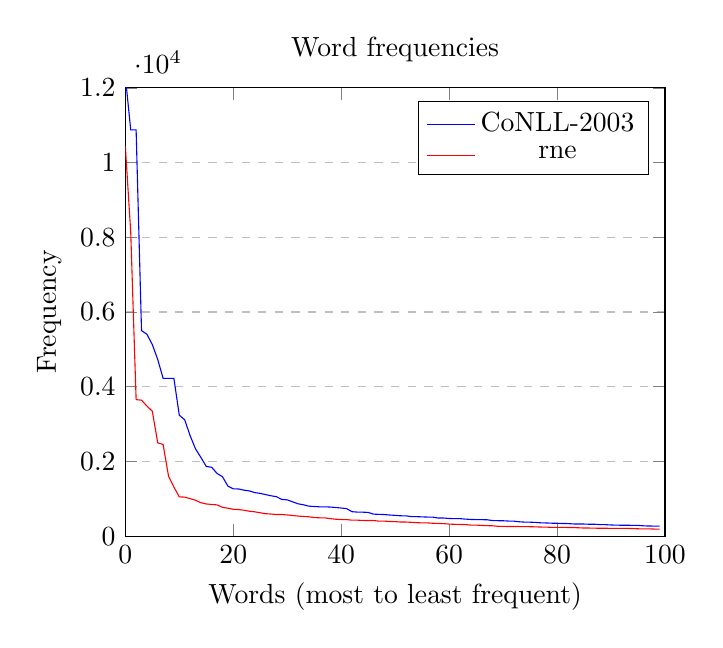
\begin{tikzpicture}
      \begin{axis}[
        title={Word frequencies},
        xmin=0, xmax=100,
        ymin=0, ymax=12000,
        ylabel={Frequency},
        xlabel={Words (most to least frequent)},
        ymajorgrids=true,
        grid style=dashed,
        legend pos=north east,
        % scaled y ticks=false,
      ]

      \addplot[color=blue, color=blue] coordinates {
        (0,12310)(1,10876)(2,10874)(3,5502)(4,5405)(5,5129)(6,4731)(7,4226)(8,4225)(9,4223)(10,3239)(11,3115)(12,2694)(13,2339)(14,2109)(15,1866)(16,1845)(17,1679)(18,1593)(19,1342)(20,1267)(21,1264)(22,1232)(23,1212)(24,1166)(25,1146)(26,1113)(27,1082)(28,1057)(29,984)(30,973)(31,920)(32,867)(33,841)(34,804)(35,796)(36,786)(37,786)(38,780)(39,768)(40,754)(41,738)(42,656)(43,645)(44,643)(45,636)(46,591)(47,584)(48,579)(49,567)(50,558)(51,546)(52,545)(53,524)(54,523)(55,517)(56,512)(57,510)(58,486)(59,486)(60,474)(61,470)(62,470)(63,457)(64,448)(65,444)(66,442)(67,441)(68,419)(69,415)(70,413)(71,405)(72,402)(73,386)(74,377)(75,375)(76,369)(77,358)(78,354)(79,348)(80,346)(81,340)(82,338)(83,328)(84,327)(85,325)(86,320)(87,319)(88,310)(89,308)(90,300)(91,296)(92,293)(93,292)(94,291)(95,289)(96,278)(97,272)(98,271)(99,271)
      };
      \addplot[color=red, color=red] coordinates {
        (0,10439)(1,8140)(2,3655)(3,3641)(4,3484)(5,3345)(6,2499)(7,2456)(8,1611)(9,1315)(10,1053)(11,1046)(12,1006)(13,963)(14,897)(15,863)(16,849)(17,838)(18,773)(19,749)(20,720)(21,713)(22,695)(23,668)(24,652)(25,626)(26,602)(27,593)(28,581)(29,580)(30,569)(31,553)(32,539)(33,527)(34,520)(35,499)(36,492)(37,490)(38,469)(39,454)(40,446)(41,444)(42,429)(43,429)(44,422)(45,420)(46,419)(47,403)(48,403)(49,394)(50,390)(51,379)(52,379)(53,371)(54,362)(55,356)(56,355)(57,346)(58,342)(59,337)(60,324)(61,318)(62,314)(63,311)(64,298)(65,297)(66,288)(67,282)(68,279)(69,265)(70,263)(71,259)(72,259)(73,258)(74,258)(75,254)(76,250)(77,245)(78,243)(79,236)(80,236)(81,235)(82,234)(83,232)(84,225)(85,219)(86,218)(87,215)(88,212)(89,212)(90,210)(91,209)(92,208)(93,208)(94,205)(95,198)(96,197)(97,196)(98,191)(99,191)
      };
      \legend{CoNLL-2003, \gls{rne}};
       
      \end{axis}
    \end{tikzpicture}
    \caption{
      Word frequencies plot for the {CoNLL-2003} dataset and the RNE dataset.
    }
    \label{fig:word_frequency_plot}
  \end{center}
\end{figure}

\subsection{Features}

Thirteen categorical features were associated with each token in the dataset. They 
are presented in Table \ref{tab:features}.

\begin{table}[h]
  \small
  \begin{center}
    \begin{tabular}{ ll }
      \toprule
      Feature & Description \\
      \midrule
      1  & Unaccented lowercase token \\
      2  & Exact gazetteer match \\
      3  & Partial gazetteer match \\
      4  & Log name gazetteer count\\
      5  & Log word gazetteer count\\
      6  & Email \\
      7  & Number \\
      8  & Honorific (Mr., Mrs., Dr., etc.)\\
      9  & URL \\
      10 & Is capitalized \\
      11 & Is a punctuation sign \\
      12 & HTML tag + parent \\
      13 & CSS class \\
      \bottomrule
    \end{tabular}
  \end{center}
  \caption{Features used in the NER on HTML dataset}
  \label{tab:features}
\end{table}

\begin{table}[h]
  \small
  \begin{center}
    \begin{tabular}{ lllll }
      \toprule
      Data file & Precision & Recall & F1 & Correct names \\
      \midrule
      Training   & 0.7316 & 0.2303 & 0.3504 & 1341 of 5822 \\ 
      Validation & 0.8474 & 0.2858 & 0.4274 & 511 of 1788 \\ 
      Test       & 0.8717 & 0.3287 & 0.4773 & 890 of 2708 \\ 
      \bottomrule
    \end{tabular}
  \end{center}
  \caption{Gazetteer coverage in each data file}
  \label{tab:gazetteer}
\end{table}

The unaccented lowercase token was used as the key for the GloVe-100 embedding lookup.
A gazetteer was constructed from a researcher list extracted from DBLP with 1,595,771
names. Table \ref{tab:gazetteer} shows the precision, recall and F1 score obtained with an
exact gazetteer matching strategy in each data file as a baseline.
Feature 2 represents an exact match of a sequence of tokens to any of the 1,595,771 
names, and feature 3 represents a partial match. Feature 4 is the rounded logarithm of 
the frequency of a token in the gazetteer, and feature 5 is the rounded logarithm of the frequency
of a token in a word corpus obtained through a random crawl on university websites.
Features 6 to 11 represent a simple regular expression match to an email, number, 
honorific, URL, capitalization or punctuation sign.

Feature 12 represents the HTML enclosing tag and its parent concatenated. Feature 13
represents all CSS classes concatenated. These features are not very useful in a general
sense, because every HTML document has a different format, so only because a named entity
occurs inside a given HTML tag in a document we cannot say it is more likely to be the case 
in other documents. However, these features can be useful for the HMM self-training strategy 
described in section \ref{sssec:self_training}. 

\section{Experiments}

We conducted experiments to evaluate sequence labeling methods of named entity 
recognition on HTML in the context of \gls{wde} using the dataset 
described in Section~\ref{sec:ner_dataset}. The tested models are described in
Table~\ref{tab:models}.

\begin{table}[h]
  \small
  \begin{center}
    \begin{tabular}{ ll }
      \toprule
      Model & Description \\
      \midrule
      hmm-1            & Regular HMM \\
      hmm-2            & HMM with $ k=2 $ \\
      hmm-3            & HMM with $ k=3 $ \\
      crf              & Linear chain conditional random fields \\
      bi-lstm-crf      & BI-LSTM-CRF model \\
      bi-lstm-crf-cnn  & BI-LSTM-CRF with CNN character representations \\
      bi-lstm-crf-lstm & BI-LSTM-CRF with LSTM character representations \\
      \bottomrule
    \end{tabular}
  \end{center}
  \caption{Model descriptions}
  \label{tab:models}
\end{table}

The evaluation of model performance was done through the precision, recall and 
F1 scores \cite{Rijsbergen1979}. Precision is the percentage of named entities found by 
the model that are correct. Recall is the percentage of named entities that are present
in the corpus and were found by the model. The F1 score is a composite measure that combines
precision and recall with the formula:

\begin{equation}
F1 = \frac{2 * precision * recall}{precision + recall}
\end{equation}

Named entities were only considered to be correct if they were a complete match of the 
corresponding entity in the dataset.

\subsection{Experiment 1: No features}

Experiment 1 aimed to evaluate the performance of sequence model with no features
besides GloVe-100 embeddings. In the case of HMMs, only the lowercase
unaccented token was used as a feature. Table \ref{tab:experiment1} 
shows the Precision (P), Recall (R), and F1-scores (F1) for this
experiment.

\begin{table}[h]
  \small
  \begin{center}
    \begin{tabular}{ lllllll }
      \toprule
      \multirow{2}{*}{Model} & \multicolumn{3}{c}{Validation} & \multicolumn{3}{c}{Test} \\
                             & \multicolumn{1}{c}{P} & \multicolumn{1}{c}{R} & \multicolumn{1}{c}{F1}
                             & \multicolumn{1}{c}{P} & \multicolumn{1}{c}{R} & \multicolumn{1}{c}{F1} \\
      \midrule
      hmm-1	       & 0.6965 & 0.5749 & 0.6299 & 0.6263 & 0.4431 & 0.5190 \\
      hmm-2	       & 0.7047 & 0.6286 & 0.6645 & 0.6480 & 0.5222 & 0.5783 \\
      hmm-3	       & 0.6127 & 0.6141 & 0.6134 & 0.5471 & 0.4634 & 0.5018 \\
      crf	       & 0.7173 & 0.6683 & 0.6920 & 0.6671 & 0.5868 & 0.6244 \\
      bi-lstm-crf      & 0.8484 & 0.9044 & 0.8755 & 0.8358 & 0.8497 & 0.8427 \\
      bi-lstm-crf-cnn  & 0.9058 & 0.9575 & 0.9309 & 0.8779 & 0.8737 & 0.8758 \\
      bi-lstm-crf-lstm & 0.9134 & 0.9435 & 0.9282 & \textbf{0.8920} & \textbf{0.8815} & \textbf{0.8867} \\
      \bottomrule
    \end{tabular}
  \end{center}
  \caption{Precision, recall and F1 in the NER on HTML dataset for models that incorporate no features}
  \label{tab:experiment1}
\end{table}

Without carefully designed features or gazetteers, HMMs and CRFs have a very 
poor performance, achieving an F1-score of only 0.5783 for HMM-2 and 0.6244 for CRF
at the test set. This is expected, since these models rely on good feature selections.

The neural models achieved high F1-scores in the test
set even with the absence of features. The plain BI-LSTM-CRF architecture improved performance 
significantly in comparison with the conventional CRF (0.8427 against 0.6244). 
Also, neural character representations boosted performance by a significant margin
reaching an F1-score of 0.8758 for CNN-based representations and 0.8867 for LSTM-based
representations. LSTM based representations were superior in modelling
morphological features, perhaps because they are able to differentiate suffixes 
and prefixes, while CNN filters are position invariant. 

The results in Experiment 1 also show that pretrained word embeddings can work 
as a kind of universal gazetteer. Words with similar embeddings are likely to 
belong to the same class. This knowledge combined with the ability to learn 
morphological features can make up for the scarcity of textual data on some 
webpages.

\subsection{Experiment 2: All features}

Experiment 2 aimed to evaluate the performance of sequence model with all
the features described in Table~\ref{tab:features}. In this experiment, we
also evaluate the self-training strategy for HMMs described in Section 
\ref{sssec:self_training}. The self trained HMMs are described with the 
suffix "+ST". Table \ref{tab:experiment2} shows the results for Experiment 2.

\begin{table}[h]
  \small
  \begin{center}
    \begin{tabular}{ lllllll }
      \toprule
      \multirow{2}{*}{Model} & \multicolumn{3}{c}{Validation} & \multicolumn{3}{c}{Test} \\
                             & \multicolumn{1}{c}{P} & \multicolumn{1}{c}{R} & \multicolumn{1}{c}{F1}
                             & \multicolumn{1}{c}{P} & \multicolumn{1}{c}{R} & \multicolumn{1}{c}{F1} \\
      \midrule
      hmm-1	         & 0.6061 & 0.7282 & 0.6616 & 0.7106 & 0.7633 & 0.7360 \\
      hmm-2	         & 0.6279 & 0.7550 & 0.6856 & 0.7521 & 0.7810 & 0.7663 \\
      hmm-3	         & 0.6573 & 0.7819 & 0.7142 & 0.7523 & 0.7795 & 0.7657 \\
      hmm-1+ST           & 0.7032 & 0.9077 & 0.7925 & 0.7522 & 0.8663 & 0.8052 \\
      hmm-2+ST           & 0.7321 & 0.9172 & 0.8143 & 0.7737 & 0.8789 & 0.8230 \\
      hmm-3+ST           & 0.7551 & 0.9172 & 0.8283 & 0.7961 & 0.8534 & 0.8237 \\
      crf	         & 0.9024 & 0.9049 & 0.9037 & 0.8751 & 0.8227 & 0.8481 \\
      bi-lstm-crf        & 0.9430 & 0.9530 & 0.9480 & 0.8998 & 0.8527 & 0.8756 \\
      bi-lstm-crf-cnn    & 0.9244 & 0.9715 & 0.9474 & 0.9017 & \textbf{0.8973} & \textbf{0.8995} \\
      bi-lstm-crf-lstm   & 0.9465 & 0.9692 & 0.9577 & \textbf{0.9108} & 0.8715 & 0.8907 \\
      \bottomrule
    \end{tabular}
  \end{center}
  \caption{Precision, recall and F1 in the NER on HTML dataset for models that incorporate all features}
  \label{tab:experiment2}
\end{table}

Conventional models like HMMs, and CRFs can become competitive with
the right selection of features and a good gazetteer, however they still lose
to the best neural model without features, demonstrating their inherent limitations.
HMMs that employed trigrams or quadrigrams (hmm-2, hmm-3) performed better than
regular HMMs. Also, we can see that the self-training strategy for HMMs improved 
the quality of the models significantly in all cases, boosting both precision and recall. 
This hints at the possibility to adapt this strategy to neural networks and boost
the performance of neural models on the NER on HTML task.

The neural models also improved a little with the addition of features. The plain BI-LSTM-CRF
model gets a closer performance to the models that employed neural character 
representations. It suggests that the LSTM and CNN character representations 
were able to learn at least part of the morphological features automatically in the
first experiment. So, when these features are added explicitly, the differences 
in performance between different neural models become less noticeable.

\section{Conclusion}

Machine-learning-based sequence labeling models provide a flexible approach to \gls{wde}, 
in contrast to more traditional methods. In simple cases, a neural
named entity tagger may be sufficient to solve the entire data extraction task. In 
other cases, the sequence tagger remains an important part of the \gls{wde} 
system, as it performs attribute labeling on data records with accuracy and flexibility.

In this article, we compared the performance of different sequence models on the task of
named entity recognition on HTML, introducing a novel dataset that is publicly available. 
We found that there are two components to the most successful models: neural based character 
representations that extract morphological features automatically, and the joint modelling 
of output labels.

We showed that a BI-LSTM-CRF neural network with LSTM-based character representations can 
be employed effectively to solve a \gls{wde} task, achieving an F1-score of 
0.8867 with no feature engineering on the faculty listings dataset.

The effective recognition of named entities on HTML is an essential step in most general 
\gls{wde} methods. The accuracy achieved by deep neural architectures even
on webpages that are very different from the plain text for which these architectures 
were initially designed shows the potential for a truly flexible approach to cross domain 
\gls{wde}.

% \bibliographystyle{named}
% \bibliography{bibfile}

% \begin{thebibliography}{}
%   \bibitem[\protect\citename{Akmajian and Lehrer }1976]{akm76}
%   Akmajian, A. and Lehrer, A. (1976) NP-like quantifiers and the
%   problem of determining the head of an NP. {\it Linguistic
%   Analysis\/} {\bf 2}: 295--313.
%   \bibitem[\protect\citename{Huddleston }1984]{hud84}
%   Huddleston, Rodney. (1984) {\it Introduction to the Grammar of
%   English}. Cambridge: Cambridge University Press.
%   \bibitem[\protect\citename{McCord }1990]{mcc90}
%   McCord, Michael C. (1990) Slot grammar: a system for simpler
%   construction of practical natural language grammars. In R.
%   Studer (ed.), {\it Natural Language and Logic: International
%   Scientific Symposium}, pp.~118--45. Lecture Notes in Computer
%   Science. Berlin: Springer-Verlag.
%   \bibitem[\protect\citename{Salton {\it et al.}\ }1990]{sal90}
%   Salton, Gerald, Zhao, Zhongnan and Buckley, Chris. (1990)
%   A simple syntactic approach for the generation of indexing
%   phrases. Technical Report 90--1137, Department of Computer
%   Science, Cornell University.
% \end{thebibliography}

\bibliographystyle{apa}

% \cite{Zhu2005,Zhu2006,Abdessalem2010,Furche2012,Furche2012a}. Usually, 

\begin{thebibliography}{}

\bibitem[\protect\citename{Kushmerick }2000]{Kushmerick2000}
Kushmerick, N. (2000) 
Wrapper induction: efficiency and expressiveness.
{\it Artificial Intelligence\/} 
{\bf 118(1-2)}: 15--68.

\bibitem[\protect\citename{Muslea, Minton and Knoblock }1999]{Muslea1999}
Muslea I., Minton S., and Knoblock C. (1999) 
A Hierarchical Approach to Wrapper Induction.
In {\it Proceedings of the Third Annual Conference on Autonomous Agents}, 
pp.~190--197, New York: ACM.

\bibitem[\protect\citename{Hsu and Dung }{1998}]{Hsu1998}
Hsu, Chun-Nan and Dung Ming-Tzung. (1998) 
Generating finite-state transducers for semi-structured data extraction from the Web.
{\it Information Systems \/}, 
{\bf 23(8)}: 521--538.

\bibitem[\protect\citename{Crescenzi, Mecca, and Merialdo }2001]{Crescenzi2001}
Crescenzi V., Mecca G., and Merialdo P. (2001)
Roadrunner: Towards automatic data extraction from large web sites.
In {\it Proceedings of the 27th International Conference on Very Large Data Bases}, 
pp. 109--118.

\bibitem[\protect\citename{Zhu, Nie, Wen, Zhang, and Ma }2005]{Zhu2005}
Zhu J., Nie Z., Wen J., Zhang B., and Ma W. (2005)
2D Conditional Random Fields for Web Information Extraction.
In {\it Proceedings of the 22Nd International Conference on Machine Learning (ICML '05)}, 
pp.~1044--1051, New York: ACM.

\bibitem[\protect\citename{Zhu, Nie, Wen, Zhang, and Ma }2006]{Zhu2006}
Zhu J., Nie Z., Wen J., Zhang B., and Ma W. (2006)
Simultaneous Record Detection and Attribute Labeling in Web Data Extraction.
In {\it Proceedings of the 12th ACM SIGKDD International Conference on Knowledge Discovery and Data Mining (KDD '06)}, 
pp.~494--503, New York: ACM.

\bibitem[\protect\citename{Abdessalem T., Cautis B., and Derouiche N. }{2010}]{Abdessalem2010}
Abdessalem T., Cautis B., and Derouiche N. (2010)
ObjectRunner: Lightweight, targeted extraction and querying of structured web data.
In {\it Proceedings of the VLDB Endowment}
{\bf 3(1-2)}: 1585--1588.

\bibitem[\protect\citename{Furche {\it et al.}\ }{2012}]{Furche2012}
Furche, T., Gottlob, G., Grasso, G., Gunes, O., Guo, X., Kravchenko, A., Orsi, G., Schallhart, C., Sellers, A., and Wang, C. (2012)
Diadem: Domain-centric, intelligent, automated data extraction methodology.
In {\it Proceedings of the 21st International Conference on World Wide Web (WWW '12 Companion)}, 
pp. 267--270, New York, ACM.

\bibitem[\protect\citename{Collobert, Weston, Bottou, Karlen, Kavukcuoglu, and Kuksa }2011]{Collobert2011}
Collobert, R., Weston, J., Bottou, L., Karlen, M., Kavukcuoglu, K. and Kuksa P. (2011)
Natural language processing (almost) from scratch.
{\it Journal of Machine Learning Research}
{\bf 12}: 2493--2537.

\bibitem[\protect\citename{Ribas, Ribeiro-Neto, de Souza e Silva, Ueda, and Ziviani }2015]{Ribas2015}
Ribas, S., Ribeiro-Neto, B., de Souza e Silva, E., Ueda, A., and Ziviani, N. (2015)
In {\it Proceedings of the 24th International Conference on World Wide Web (WWW '15 Companion)}, 
pp. 603--608, New York, ACM.

\bibitem[\protect\citename{Adelberg }1998]{Adelberg1998}
Adelberg B. (1998)
NoDoSE---a tool for semi-automatically extracting structured and semistructured data from text documents.
{\it ACM SIGMOD Record} 
{\bf 27(2)}: 283--294.

\bibitem[\protect\citename{Laender, Ribeiro-Neto, da Silva }2002a]{Laender2002a}
Laender, A., Ribeiro-Neto, B. and da Silva, A. (2002)
DEByE - Date extraction by example.
{\it Data Knowledge Engineering}
{\bf 40(2)}: 121--154.

\bibitem[\protect\citename{Califf and Mooney }1999]{Califf1999}
Califf, M. and Mooney, R. (1999)
Relational learning of pattern-match rules for information extraction.
{\it Computational Linguistics}
{\bf 4}: 9--15.

\bibitem[\protect\citename{Laender, Ribeiro-Neto, da Silva and Teixeira }2002b]{Laender2002b}
Laender, A., Ribeiro-Neto, B., da Silva, A., and Teixeira, J. (2002)
A brief survey of web data extraction tools.
{\it SIGMOD Record}
{\bf 31(2)}: 84--93.

\bibitem[\protect\citename{Hammer, McHugh and Garcia-Molin }1997]{Hammer1997}
Hammer, J., McHugh, J. and Garcia-Molin, H. (1997)
Semistructured Data: The TSIMMIS Experience.
In {\it Proceedings of the First East-European Conference on Advances in Databases and Information Systems (ADBIS'97)}
pp 22--22, Swindon, UK, BCS Learning \& Development Ltd.

\bibitem[\protect\citename{Arocena and Mendelzon}{1998}]{Arocena1999}
Gustavo~O. Arocena and Alberto~O. Mendelzon.
\newblock {WebOQL}: Restructuring documents, databases, and webs.
\newblock In {\em Proceedings of the Fourteenth International Conference on
  Data Engineering}, ICDE '98, pages 24--33, Washington, DC, USA, 1998. IEEE
  Computer Society.



\bibitem[\protect\citename{Akbik \bgroup \em et al.\egroup
  }{2018}]{Akbik2018}
Alan Akbik, Duncan Blythe, and Roland Vollgraf.
\newblock Contextual string embeddings for sequence labeling.
\newblock In {\em Proceedings of the 27th International Conference on
  Computational Linguistics}, pages 1638--1649, Santa Fe, New Mexico, USA,
  August 2018. Association for Computational Linguistics.

\bibitem[\protect\citename{Baevski \bgroup \em et al.\egroup
  }{2019}]{Baevski2019}
Alexei Baevski, Sergey Edunov, Yinhan Liu, Luke Zettlemoyer, and Michael Auli.
\newblock Cloze-driven pretraining of self-attention networks.
\newblock {\em Preprint arXiv:1903.07785}, 2019.

\bibitem[\protect\citename{Bikel \bgroup \em et al.\egroup
  }{1999}]{Bikel1999}
Daniel~M. Bikel, Richard Schwartz, and Ralph~M. Weischedel.
\newblock An algorithm that learns what's in a name.
\newblock {\em Machine Learning}, 34(1):211--231, Feb 1999.

\bibitem[\protect\citename{Borthwick \bgroup \em et al.\egroup
  }{1998}]{Borthwick1998}
Andrew Borthwick, John Sterling, Eugene Agichtein, and Ralph Grishman.
\newblock Exploiting diverse knowledge sources via maximum entropy in named
  entity recognition.
\newblock In {\em Proceedings of the Sixth Workshop on Very Large Corpora},
  pages 152--160. Association for Computational Linguistics, 1998.

\bibitem[\protect\citename{Caruana \bgroup \em et al.\egroup
  }{2000}]{Caruana2000}
Rich Caruana, Steve Lawrence, and Lee Giles.
\newblock Overfitting in neural nets: Backpropagation, conjugate gradient, and
  early stopping.
\newblock In {\em Proceedings of the 13th International Conference on Neural
  Information Processing Systems}, NIPS'00, pages 381--387, Cambridge, MA, USA,
  2000. MIT Press.

\bibitem[\protect\citename{Chang and Kuo}{2004}]{Chang2004}
Chia~Hui Chang and Shih~Chien Kuo.
\newblock {OLERA: Semisupervised Web-data extraction with visual support}.
\newblock {\em IEEE Intelligent Systems}, 19(6):56--64, 2004.

\bibitem[\protect\citename{Chang \bgroup \em et al.\egroup
  }{2001}]{Chang2001}
C.H. Chang, C.H. Chang, S.C. Lui, and S.C. Lui.
\newblock {IEPAD: information extraction based on pattern discovery}.
\newblock {\em Proceedings of the 10th international conference on World Wide
  Web}, pages 681--688, 2001.

\bibitem[\protect\citename{Chang \bgroup \em et al.\egroup
  }{2006}]{Chang2006}
Chia-Hui Chang, Mohammed Kayed, Moheb~Ramzy Girgis, and Khaled~F Shaalan.
\newblock {A Survey of Web Information Extraction Systems}.
\newblock {\em IEEE Transactions on Knowledge and Data Engineering},
  18(10):1411--1428, 2006.

\bibitem[\protect\citename{Devlin \bgroup \em et al.\egroup
  }{2018}]{Devlin2018}
Jacob Devlin, Ming-Wei Chang, Kenton Lee, and Kristina Toutanova.
\newblock {BERT}: Pre-training of deep bidirectional transformers for language
  understanding.
\newblock {\em Preprint arXiv:1810.04805}, 2018.

\bibitem[\protect\citename{Dong \bgroup \em et al.\egroup
  }{2014}]{Dong2014}
Xin Dong, Evgeniy Gabrilovich, Geremy Heitz, Wilko Horn, Ni~Lao, Kevin Murphy,
  Thomas Strohmann, Shaohua Sun, and Wei Zhang.
\newblock {Knowledge Vault: a web-scale approach to probabilistic knowledge
  fusion}.
\newblock {\em Proceedings of the 20th ACM SIGKDD international conference on
  Knowledge discovery and data mining - KDD '14}, pages 601--610, 2014.

\bibitem[\protect\citename{Ferrara and Baumgartner}{2011}]{Ferrara2011}
Emilio Ferrara and Robert Baumgartner.
\newblock {Automatic wrapper adaptation by tree edit distance matching}.
\newblock {\em Smart Innovation, Systems and Technologies}, 8:41--54, 2011.

\bibitem[\protect\citename{Ferrara \bgroup \em et al.\egroup
  }{2014}]{Ferrara2014}
Emilio Ferrara, Pasquale {De Meo}, Giacomo Fiumara, and Robert Baumgartner.
\newblock {Web data extraction, applications and techniques: A survey}.
\newblock {\em Knowledge-Based Systems}, 70:301--323, 2014.

\bibitem[\protect\citename{Florian \bgroup \em et al.\egroup
  }{2003}]{Florian2003}
Radu Florian, Abe Ittycheriah, Hongyan Jing, and Tong Zhang.
\newblock Named entity recognition through classifier combination.
\newblock In {\em Proceedings of the Seventh Conference on Natural Language
  Learning at HLT-NAACL 2003}, pages 168--171, 2003.

\bibitem[\protect\citename{Freitag and Mccallum}{1999}]{Freitag1999}
Dayne Freitag and Andrew~Kachites Mccallum.
\newblock {Information Extraction with HMMs and Shrinkage}.
\newblock In {\em Proceedings of the AAAI-99 Workshop on Machine Learning for
  Information Extraction}, pages 31--36. AAAI Press, 2 1999.

\bibitem[\protect\citename{Freitag and McCallum}{2000}]{Freitag2000}
Dayne Freitag and Andrew McCallum.
\newblock {Information Extraction with HMM Structures Learned by Stochastic
  Optimization}.
\newblock In {\em Proceedings of the Seventeenth National Conference on
  Artificial Intelligence and Twelfth Conference on Innovative Applications of
  Artificial Intelligence}, pages 584--589. AAAI Press, 2000.

\bibitem[\protect\citename{Freitag}{1998}]{Freitag1998}
Dayne Freitag.
\newblock {Information Extraction from HTML: Application of a General Machine
  Learning Approach}.
\newblock In {\em Proceedings of the Fifteenth National/Tenth Conference on
  Artificial Intelligence/Innovative Applications of Artificial Intelligence},
  AAAI '98/IAAI '98, pages 517--523, Menlo Park, CA, USA, 1998. American
  Association for Artificial Intelligence.

\bibitem[\protect\citename{Hochreiter and
  Schmidhuber}{1997}]{Hochreiter1997}
Sepp Hochreiter and J\"{u}rgen Schmidhuber.
\newblock Long short-term memory.
\newblock {\em Neural Computation}, 9(8):1735--1780, November 1997.

\bibitem[\protect\citename{Hogue and Karger}{2005}]{Hogue2005}
Andrew Hogue and David Karger.
\newblock {Thresher: Automating the Unwrapping of Semantic Content from the
  World Wide Web}.
\newblock In {\em Proceedings of the 14th International Conference on World
  Wide Web}, WWW '05, pages 86--95, New York, NY, USA, 2005. ACM.

\bibitem[\protect\citename{Huang \bgroup \em et al.\egroup
  }{2015}]{Huang2015}
Zhiheng Huang, Wei Xu, and Kai Yu.
\newblock Bidirectional {LSTM-CRF} models for sequence tagging.
\newblock {\em CoRR}, abs/1508.01991, 2015.

\bibitem[\protect\citename{Kr{\"{u}}pl \bgroup \em et al.\egroup
  }{2005}]{Krupl2005}
Bernhard Kr{\"{u}}pl, Marcus Herzog, and Wolfgang Gatterbauer.
\newblock {Using visual cues for extraction of tabular data from arbitrary HTML
  documents}.
\newblock {\em Special interest tracks and posters of the 14th international
  conference on World Wide Web - WWW '05}, pages 1000----1001, 2005.

\bibitem[\protect\citename{Lafferty \bgroup \em et al.\egroup
  }{2001}]{Lafferty2001}
John~D. Lafferty, Andrew McCallum, and Fernando C.~N. Pereira.
\newblock Conditional random fields: Probabilistic models for segmenting and
  labeling sequence data.
\newblock In {\em Proceedings of the Eighteenth International Conference on
  Machine Learning}, ICML '01, pages 282--289, San Francisco, CA, USA, 2001.
  Morgan Kaufmann Publishers Inc.

\bibitem[\protect\citename{Lample \bgroup \em et al.\egroup
  }{2016}]{Lample2016}
Guillaume Lample, Miguel Ballesteros, Sandeep Subramanian, Kazuya Kawakami, and
  Chris Dyer.
\newblock Neural architectures for named entity recognition.
\newblock {\em CoRR}, abs/1603.01360, 2016.

\bibitem[\protect\citename{Li and Gray}{2000}]{Li2000}
Jia Li and Robert~M. Gray.
\newblock {\em Image Segmentation and Compression Using Hidden Markov Models}.
\newblock Kluwer Academic Publishers, Norwell, MA, USA, 2000.

\bibitem[\protect\citename{Liu and Nocedal}{1989}]{Liu1989}
Dong~C. Liu and Jorge Nocedal.
\newblock On the limited memory bfgs method for large scale optimization.
\newblock {\em Mathematical Programming}, 45(1):503--528, Aug 1989.

\bibitem[\protect\citename{Liu \bgroup \em et al.\egroup
  }{2000}]{Liu2000}
L.~Liu, C.~Pu, and W.~Han.
\newblock {XWRAP: an XML-enabled wrapper construction system for Web
  information sources}.
\newblock {\em Proceedings of 16th International Conference on Data
  Engineering}, pages 611--621, 2000.

\bibitem[\protect\citename{Ma and Hovy}{2016}]{Ma2016}
Xuezhe Ma and Eduard Hovy.
\newblock End-to-end sequence labeling via bi-directional {LSTM}-{CNN}s-{CRF}.
\newblock In {\em Proceedings of the 54th Annual Meeting of the Association for
  Computational Linguistics (Volume 1: Long Papers)}, pages 1064--1074, Berlin,
  Germany, August 2016. Association for Computational Linguistics.

\bibitem[\protect\citename{McCallum and Li}{2003}]{McCallum2003}
Andrew McCallum and Wei Li.
\newblock Early results for named entity recognition with conditional random
  fields, feature induction and web-enhanced lexicons.
\newblock In {\em Proceedings of the Seventh Conference on Natural Language
  Learning at HLT-NAACL 2003 - Volume 4}, CONLL '03, pages 188--191,
  Stroudsburg, PA, USA, 2003. Association for Computational Linguistics.

\bibitem[\protect\citename{McCallum \bgroup \em et al.\egroup
  }{2000}]{McCallum2000}
Andrew McCallum, Dayne Freitag, and Fernando C.~N. Pereira.
\newblock Maximum entropy markov models for information extraction and
  segmentation.
\newblock In {\em Proceedings of the Seventeenth International Conference on
  Machine Learning}, ICML '00, pages 591--598, San Francisco, CA, USA, 2000.
  Morgan Kaufmann Publishers Inc.

\bibitem[\protect\citename{Pennington \bgroup \em et al.\egroup
  }{2014}]{Pennington2014}
Jeffrey Pennington, Richard Socher, and Christopher~D. Manning.
\newblock Glove: Global vectors for word representation.
\newblock In {\em Empirical Methods in Natural Language Processing (EMNLP)},
  pages 1532--1543, 2014.

\bibitem[\protect\citename{Peters \bgroup \em et al.\egroup
  }{2018}]{Peters2018}
Matthew Peters, Mark Neumann, Mohit Iyyer, Matt Gardner, Christopher Clark,
  Kenton Lee, and Luke Zettlemoyer.
\newblock Deep contextualized word representations.
\newblock In {\em Proceedings of the 2018 Conference of the North {A}merican
  Chapter of the Association for Computational Linguistics: Human Language
  Technologies, Volume 1 (Long Papers)}, pages 2227--2237, New Orleans,
  Louisiana, June 2018. Association for Computational Linguistics.

\bibitem[\protect\citename{Rabiner}{1990}]{Rabiner1990}
Lawrence~R. Rabiner.
\newblock {\em {Readings in Speech Recognition. Chapter: A Tutorial on Hidden
  Markov Models and Selected Applications in Speech Recognition}}.
\newblock Morgan Kaufmann Publishers Inc., San Francisco, CA, USA, 1990.

\bibitem[\protect\citename{Ramshaw and Marcus}{1999}]{Ramshaw1999}
L.~A. Ramshaw and M.~P. Marcus.
\newblock {\em Text Chunking Using Transformation-Based Learning}, pages
  157--176.
\newblock Springer Netherlands, Dordrecht, 1999.

\bibitem[\protect\citename{Ratnaparkhi}{1998}]{Ratnaparkhi1998}
Adwait Ratnaparkhi.
\newblock {\em Maximum Entropy Models for Natural Language Ambiguity
  Resolution}.
\newblock PhD thesis, Philadelphia, PA, USA, 1998.
\newblock AAI9840230.

\bibitem[\protect\citename{Rijsbergen}{1979}]{Rijsbergen1979}
C.~J.~Van Rijsbergen.
\newblock {\em Information Retrieval}.
\newblock Butterworth-Heinemann, Newton, MA, USA, 2nd edition, 1979.

\bibitem[\protect\citename{Sahuguet and Azavant}{1999}]{Sahuguet1999}
Arnaud Sahuguet and Fabien Azavant.
\newblock {Building Light-Weight Wrappers for Legacy Web Data-Sources Using
  W4F}.
\newblock In {\em Proceedings of the 25th International Conference on Very
  Large Data Bases}, VLDB '99, pages 738--741, San Francisco, CA, USA, 1999.
  Morgan Kaufmann Publishers Inc.

\bibitem[\protect\citename{Sarawagi}{2008}]{Sarawagi2008}
Sunita Sarawagi.
\newblock {Information extraction}.
\newblock {\em Foundations and Trends in Databases}, 1(3):261--377, 2008.

\bibitem[\protect\citename{Schulz \bgroup \em et al.\egroup
  }{2016}]{Schulz2016}
Andreas Schulz, J{\"{o}}rg L{\"{a}}ssig, and Martin Gaedke.
\newblock {Practical web data extraction: Are we there yet? --- A short
  survey}.
\newblock {\em IEEE/WIC/ACM International Conference on Web Intelligence (WI),
  2016}, pages 562----567, 2016.

\bibitem[\protect\citename{Shi \bgroup \em et al.\egroup
  }{2015}]{Shi2015}
Shengsheng Shi, Chengfei Liu, Yi~Shen, Chunfeng Yuan, and Yihua Huang.
\newblock {AutoRM: An effective approach for automatic Web data record mining}.
\newblock {\em Knowledge-Based Systems}, 89:314--331, 2015.

\bibitem[\protect\citename{Soderland}{1999}]{Soderland1999}
Stephen Soderland.
\newblock {Learning Information Extraction Rules for Semi-Structured and Free
  Text}.
\newblock {\em Machine Learning}, 34(1):233--272, 1999.

\bibitem[\protect\citename{Sundheim}{1991}]{Sundheim1991}
Beth~M. Sundheim.
\newblock Overview of the third message understanding evaluation and
  conference.
\newblock In {\em Proceedings of the 3rd Conference on Message Understanding},
  MUC3 '91, pages 3--16, Stroudsburg, PA, USA, 1991. Association for
  Computational Linguistics.

\bibitem[\protect\citename{Tjong Kim~Sang and
  De~Meulder}{2003}]{KimSang2003}
Erik~F. Tjong Kim~Sang and Fien De~Meulder.
\newblock {Introduction to the CoNLL-2003 Shared Task: Language-independent
  Named Entity Recognition}.
\newblock In {\em Proceedings of the Seventh Conference on Natural Language
  Learning at HLT-NAACL 2003 - Volume 4}, CONLL '03, pages 142--147,
  Stroudsburg, PA, USA, 2003. Association for Computational Linguistics.

\bibitem[\protect\citename{Varlamov and Turdakov}{2016}]{Varlamov2016}
M.~I. Varlamov and D.~Yu. Turdakov.
\newblock {A survey of methods for the extraction of information from Web
  resources}.
\newblock {\em Programming and Computer Software}, 42(5):279--291, 2016.

\end{thebibliography}
\end{document}
